\documentclass[11pt]{article}
\usepackage{times}
\usepackage{graphicx}
\usepackage{amsmath}
\usepackage{amssymb}
\usepackage{cite}
\usepackage{color}
\usepackage[margin=1in]{geometry}
\usepackage{bm}
\usepackage{cleveref}
\usepackage[font=small,labelfont=bf]{caption}
\usepackage{subcaption}
\captionsetup[subfigure]{subrefformat=simple,labelformat=simple}
\renewcommand\thesubfigure{(\alph{subfigure})}
\geometry{a4paper}
\usepackage{float}
%\usepackage{cite}
\newcommand{\beginsupplement}{%
  \setcounter{table}{0}
  \renewcommand{\thetable}{S\arabic{table}}%
  \setcounter{figure}{0}
  \renewcommand{\thefigure}{S\arabic{figure}}%
}
\usepackage{array}
\newcolumntype{L}[1]{>{\raggedright\let\newline\\\arraybackslash\hspace{0pt}}m{#1}}
\newcolumntype{C}[1]{>{\centering\let\newline\\\arraybackslash\hspace{0pt}}m{#1}}
\newcolumntype{R}[1]{>{\raggedleft\let\newline\\\arraybackslash\hspace{0pt}}m{#1}}

\begin{document}
\title{{\color{blue}Tunable} collective behavior in active cytoskeletal assemblies}
\author{Simon L. Freedman, Shiladitya Banerjee, Glen M. Hocky, Aaron R. Dinner}
\date{}
\maketitle
\begin{abstract}
Cells {\color{red}can} modulate the mechanical properties of the cytoskeleton in remarkable ways to maintain structural integrity, move and divide. This behavior is achieved through {\color{red}dynamic} control of structural elements, including crosslinking proteins, {\color{red}bundling agents}, as well as {\color{red}molecular} motors that generate {\color{red}active} stresses and {\color{red}regulate intracellular} transport. {\em In vitro} {\color{red}model systems} using a small subset of {\color{red}purified} proteins have {\color{red}revealed the minimal} components necessary to confer this wide range of {\color{red}mechanical} behaviors, {\color{red}but have so far not been rigorously tested in simulations}. {\color{red}Here, using agent-based computational modeling, we investigate the collective dynamics of disordered cytoskeletal assemblies}, consisting of semi-flexible {\color{red}filaments}, dynamic crosslinkers, and molecular motors. {\color{red}By tuning the properties of individual cytoskeletal elements}, such as filament length, crosslinker stiffness or motor kinetics, {\color{red}we explore the collective phases of actomyosin networks across dynamic regimes previously inaccessible by experiments. Our work elucidates the diverse pathways for cytoskeletal contractility, polarity organization, and molecular transport, and provides testable predictions for future experiments on reconstituted cytoskeletal assemblies}. 
\end{abstract}

\section*{Introduction} 
The actin cytoskeleton serves as a {\color{red}dynamic} scaffold that allows {\color{red}eukaryotic} cells to {\color{red}actively change shape, move} and {\color{red}adapt} to their {\color{red}micro-}environment. Although {\color{red}the cell cytoskeleton constitutes} a complex network of protein-protein interactions, {\em in vitro} {\color{red}model systems have revealed the minimal set} of components required to exhibit a wide range of {\color{red}active mechanical} behaviors including contractility and {\color{red}polarity organization}{\color{blue}\cite{stricker2010, murrell2012} - need to revise this}. In this work, we {\color{red}investigate} the range of {\color{red}collective} behaviors {\color{red}accessible} to a {\color{red}minimal} system consisting of {\color{red}cytoskeletal} filaments, crosslinking proteins, and active {\color{red}molecular} motors. {\color{red}While previous studies have shed light on the mechanisms of contractility and self-organization in minimal cytoskeletal systems (cite)}, a necessary limitation is the difficulty to precisely control the properties of {\color{red}individual cytoskeletal systems}. For {\color{red}instance, it is poorly understood how variations in} filament stiffness, length, crosslinker {\color{red}geometry} and affinity {\color{red}control emergent properties of cytoskeletal assemblies}. {\color{red}Here we} present an {\color{red}agent-based model of cytoskeleton}, {\color{red}using} non-equilibrium molecular dynamics simulations, that can efficiently explore the {\color{red}collective} phases of {\color{red}crosslinked actomyosin networks}. {\color{red}Our agent-based} model {\color{red}is ideal for elucidating} the relationship between protein-protein interactions {\color{red}at the microscale} and the {\color{red}collective} mechanical {\color{red}behavior} of the {\color{red}assembly}. {\color{red}Furthermore, our dynamic simulations} enable us to learn {\color{red}how active networks sample through dynamic states}, and how intermediate mesoscopic structures {\color{red}may} tune network functionality {\color{red}at cellular scales}.
\par

{\color{red}Actomyosin contractility has been extensively studied} in {\color{red}the context of} muscle cells, where actin filaments are arranged in {\color{red}a sarcomeric fashion}, enabling myosin {\color{red}minifilaments} to {\color{red}translocate} anti-parallel actin filaments, resulting {\color{red}in active} muscle contraction\cite{huxley1969}. However, the cytoskeleton of nonmuscle cells {\color{red}exhibit} no inherent ordering of actin, {\color{red}where F-actin buckling has been shown to coordinate long-range contractile behavior} {\color{blue}\cite{murrell2012, stam2015, murrell2015} definitely cite Lenz et al}.
Recent {\color{red}\it in vitro} studies \cite{murrell2012, murrell2014} {\color{red}using} reconstituted networks of actin and myosin, {\color{red}have revealed} how changing {\color{red}myosin} concentrations and {\color{red}F-actin properties} affect the ability of disordered {\color{red}networks} to contract and form static structures. For {\color{red}instance}, at low
motor densities, the {\color{red}actin network behaves as non-contractile, resulting} in {\color{red}long-distance translocation of} myosin along {\color{red}actin tracks}\cite{burov2013} Above a
critical density, myosin {\color{red}motors cooperatively} contract the {\color{red}actin} network\cite{murrell2014}. {\color{red}Additionally, it has been shown that} actin binding proteins (crosslinkers) such as filamin, scruin, and $\alpha$-actinin, {\color{red}can profoundly affect} long-range force propagation as well as {\color{red}the mechanical stability of actin} bundles and networks\cite{gardel2004, murrell2012, murrell2014, murrell2015}. {\color{red}While} these experiments {\color{red}are beginning to suggest} the phase {\color{red}space of collective behavior in} active networks, {\color{red}agent-based simulations can explore in a controlled fashion how} myosin density \cite{murrell2012}, actin bundle rigidity \cite{murrell2012}, and cross-linker density\cite{murrell2014} {\color{red}are able to modulate} structure formation and force generation within the {\color{red}cell} cytoskeleton.  
%\par

%These \textit{in vitro} experiments have also been used to probe the underlying
%mechanisms that control the ensemble network behavior. 
%To date, results strongly suggest that actin filament buckling and severing as well as relative actin and myosin sliding
%are all necessary for network contraction \cite{murrell2012, murrell2014}.
\par
To probe the microscopic origins of these complex {\color{red}collective processes}, we {\color{red}propose} an {\color{red}agent-based} simulation model, motivated by both {\em in vitro} experiments as well as {\color{red}{\it in vivo} mechanical studies on} actin and myosin {\color{red}(cite)}. {\color{red}While some of the previous computational} models were designed to understand the rheology of crosslinked actin networks 
\cite{mackintosh1995,head2003,wilhelm2003,kim2009}, {\color{red}others have investigated the collective} motion of motors 
with {\color{red}on cytoskeletal tracks} \cite{nedelec2007,erdmann2012,stam2015}. {\color{red}Other coarse-grained modeling approaches} have shown how disordered assemblies of filaments and motors collectively form asters \cite{gordon2012} or 
contract {\color{red}at network level}\cite{wang2012,dasanyake2011,kim2014,ennomani2016}. Our model {\color{red}incorporates} many of the {\color{red}essential} features of {\color{red}previous modeling work}. We use the {\color{red}worm-like chain model} for an actin filament, {\color{red}with both} bending and stretching {\color{red}energies}, by initializing crosslinkers at {\color{red}filament} intersections to {\color{red}generate} well connected networks \cite{head2003}. {\color{red}However,} in contrast to Ref. \cite{head2003, dasanyake2011}, we simulate non-equilibrium dynamics, including {\color{red}thermal} fluctuations {\color{red}as well as stochastic} binding/unbinding {\color{red}kinetics of} myosins and cross linkers.  
%We have used predictions from \cite{stam2015} to {\color{red}estimate the} numerical parameters for the binding kinetics of a myosin mini-filament as they relate to a single myosin head. 
Force propagation rules and binding kinetics {\color{red}are} similar to {\color{red}previous models}
\cite{nedelec2007, gordon2012}, but with {\color{red}minor} differences in {\color{red}their implementation that improves the overall computational efficiency}. {\color{blue}SB: can we say this?}
\par
{\color{red}We accurately} bench-mark {\color{red}our simulations} to reproduce {\color{red}the well}-known experimental results for actin
filament {\color{red}dynamics}, {\color{red}as well as the collective behavior} of crosslinked actin and myosin {\color{red}driven} active networks. 
We {\color{red}quantitatively} reproduce {\color{red}the experimentally measured} spatio-temporal fluctuations {\color{red}in single} actin filaments. 
For passive crosslinked networks, we {\color{red}recover the well-established} stress-strain relationships {\color{red}measured} for {\color{red}semiflexible polymer} networks {\color{red}(cite)}. For active networks, we reproduce {\color{red}the experimentally observed} velocity distributions of actin filaments in an {\color{red}actomyosin} motility assay. These results demonstrate that {\color{red}our simulations robustly} capture {\color{red}several} key properties of cytoskeletal networks within a single {\color{red}agent-based} model. 
%which has not been optimized to reproduce any particular set of experiments. 
\par 
We then show that {\color{red}our} simulations predict {\color{red}diverse collective} dynamical behaviors {\color{red}in cytoskeletal assemblues}, {\color{red}by tuning} properties of {\color{red}individual} filaments, crosslinkers and motors. We find that crosslinker affinity modulates filament bundling and network coarsening in a {\color{red}biphasic} manner. We {\color{red}further} show that crosslinker stiffness {\color{red}can tune} the strain stiffening response of {\color{red}actin} networks in a simulated rheology experiment. We {\color{red}quantify} motor-dependent contraction {\color{red}in active networks} {\color{red}and predict how} he concentration of motors control {\color{red}actin} polarity sorting. These results {\color{red}suggest how actomyosin} contractility {\color{red}emerges from} a competition between bundling and polarity sorting.We {\color{red}characterize} how variations in {\color{red}actin} filament length, motor density, and motor-filament binding affinity can {\color{red}alter motor cooperativity} to translocate actin filaments, which may have implications for optimizing the {\color{red}observed dynamics of} polarity sorting and contractility. {\color{red}Collectively our work} demonstrates how ensembles of randomly oriented actin filaments and crosslinkers can be rearranged by myosin motors to form tunable structures with distinct biophysical and mechanical functionalities.

%Using this model we successfully explore canonical F-actin experiments, such as the motility assay and crosslinked network rheology, and show how tuning the microscopic parameters of these experiments can yield a variety of biomechanically distinct macroscopic structures.


%The collective activity of many-particle systems where pair-wise particle interactions are well understood can be elucidated via molecular dynamics simulations. A biomolecular example involves the proteins actin and myosin in the cytoskeleton of non-muscle cells. In that environment, actin monomers polymerize into polar actin filaments (F-actin) which are microns long and nanometers thick, and myosin motor proteins aggregate onto $0.4\mu m$ long backbones to form myosin minifilaments \cite{niederman1975}. For precessive motors, such as myosin II, the binding of myosin to actin, followed by ATP hydrolysis and subsequent unbinding, results in the relative motion of myosin with respect to actin toward the positive (barbed) end of an actin filament. In the cytoskeleton, this motion drives many biological processes, including endocytosis, cell-division and maintenance of cell shape
%The mechanism through which myosin can walk on actin has been extensively studied in muscle cells, where actin
%filaments are arranged in parallel bundles called sarcomeres. A myosin filament binds to two antipolar
%sarcomeres, walks toward the barbed end of both, and the tension along the myosin pulls the 
%sarcomeres together, resulting in muscle contraction\cite{huxley1969}. 
%However, in the cytoskeleton of nonmuscle cells, there is no inherent ordering of actin or myosin filaments, so while
%interactions between individual myosin and actin filaments exist, how 
%they act in concert to produce a variety of behaviors is an active area of research \cite{murrell2012, stam2015, murrell2015}. 
{\color{blue}SB: the intro currently focuses on in vitro (all actin) and in silico studies. It ignores in vivo studies as well as comparisons with active gel theories. We should try broadening the scope here.}
\section*{Results}
{\color{red}An essential mechanical} function of actomyosin networks is their contractility, which {\color{red}coordinates a variety of cellular processes including}, muscle
contraction, cell motility and division. 
That these complex macroscopic mechanisms arise stochastically from simple microscopic interactions suggests the ability
to engineer materials with controllable network topologies and dynamics. 
Recently, {\it in-vitro} experiments of
reconstituted actomyosin networks have demonstrated this controllable architecture by varying motor density and
crosslinker density, and showing how they affect contractility\cite{murrell2012, murrell2014}. Our model shows a similar dependence of 
{\color{red}network} contractility on motor density. 
Additionally, {\color{red}we demonstrate tunability between} two {\color{red}modes of network} organization: bundling, in which dynamics
crosslinkers pin filaments into robust networks, and polarity sorting, by which motors {\color{red}organize} filaments {\color{red}into structures of uniform} polarity. 
\par
{\color{red}For} computational efficiency, we coarse grain actin filaments and
crosslinker proteins at length scales relevant for network behavior. Actin filaments are
modeled as polar worm-like chains (WLC) such that one end of the chain represents the barbed end of a filament and the
other end represents its pointed end. Crosslinkers are modeled as Hookean springs such
that both ends of the spring (heads) can bind and unbind from filaments. 
Experiments have shown that adding crosslinkers to assemblies of F-actin yields actin bundles \cite{gardel2004, murrell2012, murrell2014}
and that increasing crosslinker density can increase the length scale of contraction \cite{murrell2012}. {\color{red}We} show that 
varying the stiffness of these springs {\color{red}modulates} the rheology 
of an assembly of crosslinkers and filaments, while varying the binding affinity affects the magnitude of actin bundling. We {\color{red}present a two-dimensional} model {\color{red}for actomyosin}, similar to the {\color{red}thin}, quasi-2D reconstituted networks of actomyosin. This setup is sufficient to reproduce structures of biological interest, and allows us to simulate larger systems for longer times. 
Because we use a 2D system to {\color{red}model} a 3D experiment, we exclude the steric interactions of filaments and crosslinkers, to {\color{red}allow} for
some of the freedom lost from the reduction in dimensionality.

\subsection*{Crosslink turnover modulates bundling of filament networks}
The rapid binding and unbinding of crosslinking proteins from actin
filaments can reorganize initially disordered filament {\color{red}networks} into thick bundled networks. 
This behavior is distinct from motor-driven contractility, because the overall network structure {\color{red}coarsens} without
{\color{red}any active force generation}. {\color{red}Here} we tune this bundling mechanism by
changing the crosslinker-filament binding affinity. 
\par
To demonstrate this behavior, thirteen simulations were initialized with 500 worm-like chain filaments of length 15 $\mu$m, scattered 
on a 75 $\mu$m$\times$75 $\mu$m simulation cell, and 0.15 $\mu$m long crosslinkers {\color{red}are placed} at filament-filament intersections. 
The assemblies {\color{red}are} then evolved via Brownian dynamics for 200 s.   
Each simulation had a different dissociation rate for crosslinkers $k^\text{off}_\text{cl}$ varying
logarithmically between 0-1800 s$^{-1}$. The results are shown in \Cref{fig:bundle}. 
\par
\begin{figure}
  \centering
  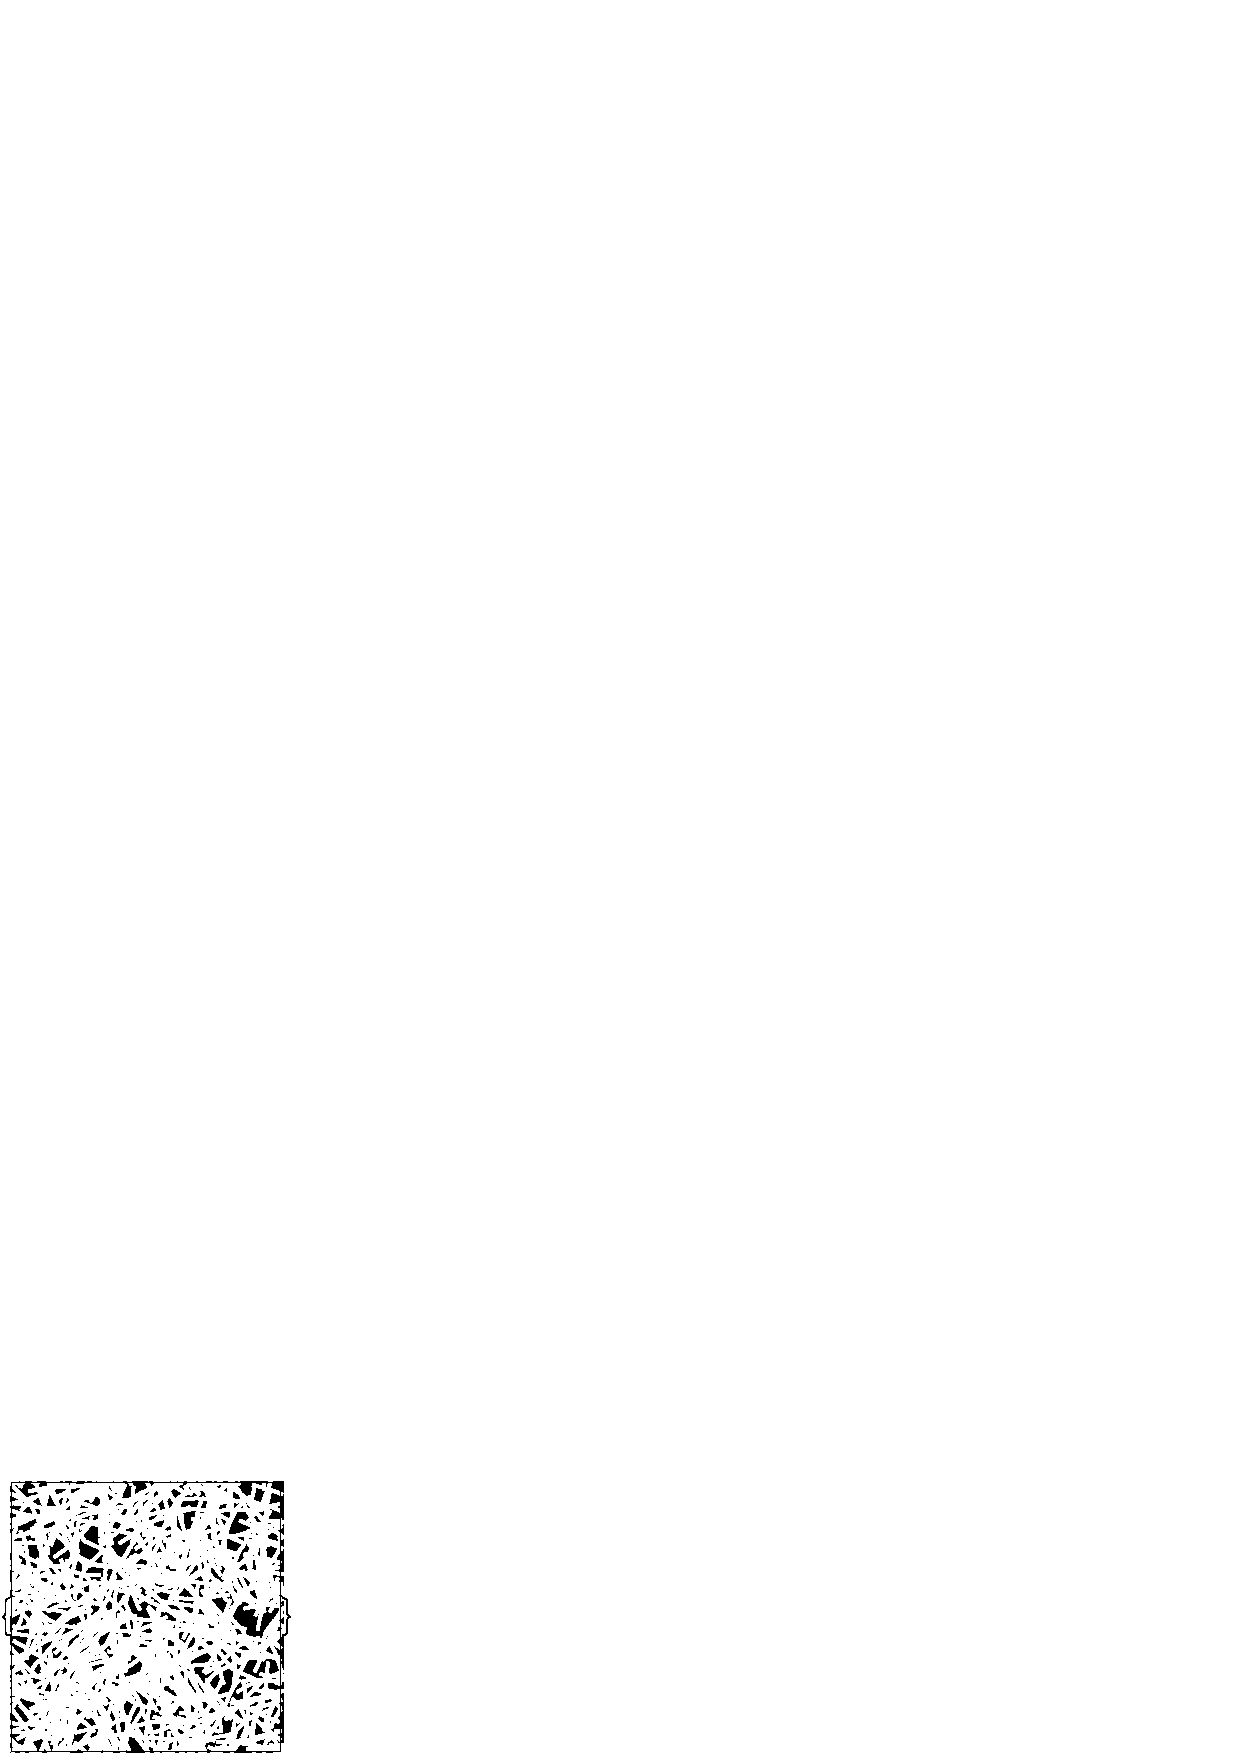
\includegraphics[width=0.6\columnwidth]{figs/t0.pdf}
  \caption{\label{fig:t0}Initial configuration of actin filaments (red) for 
  (A) assemblies which initially have crosslinkers (yellow, one third shown) placed at intersections and 
  (B) assemblies with motors $\rho_m=0.1\ \mu$m$^{-2}$ (white) scattered throughout. {\color{blue}SB: can we move fig. 8A here?}}
\end{figure}
The {\color{red}degree} of bundling {\color{red}can be quantified} by the radial
distribution function of actin filaments, $g(r) = P(r)/(2\pi r \delta r\rho)$, where $P(r)$ is the probability that two beads on different filaments are {\color{red}separated by} a distance $r$, $\delta r =0.05\ \mu$m is the bin size and $\rho = 500/(75\ \mu m)^2$ is the number density. As {\color{red}shown} in \Cref{fig:bundle}C-D, the relationship between $k^\text{off}_\text{cl}$ and $g(r)$ is non-monotonic. A {\color{red}low} disassociation rate {\color{red}does} not allow for significant restructuring from the initially random configuration, {\color{red}while} a {\color{red}high} disassociation rate {\color{red}does} not yield {\color{red}long-lived} stable structures. However, at intermediate values of $k^\text{off}_\text{cl}$, {\color{red}the filaments self-assemble into} a stable, thickly bundled network.
\par
\begin{figure}[h]
  \centering
  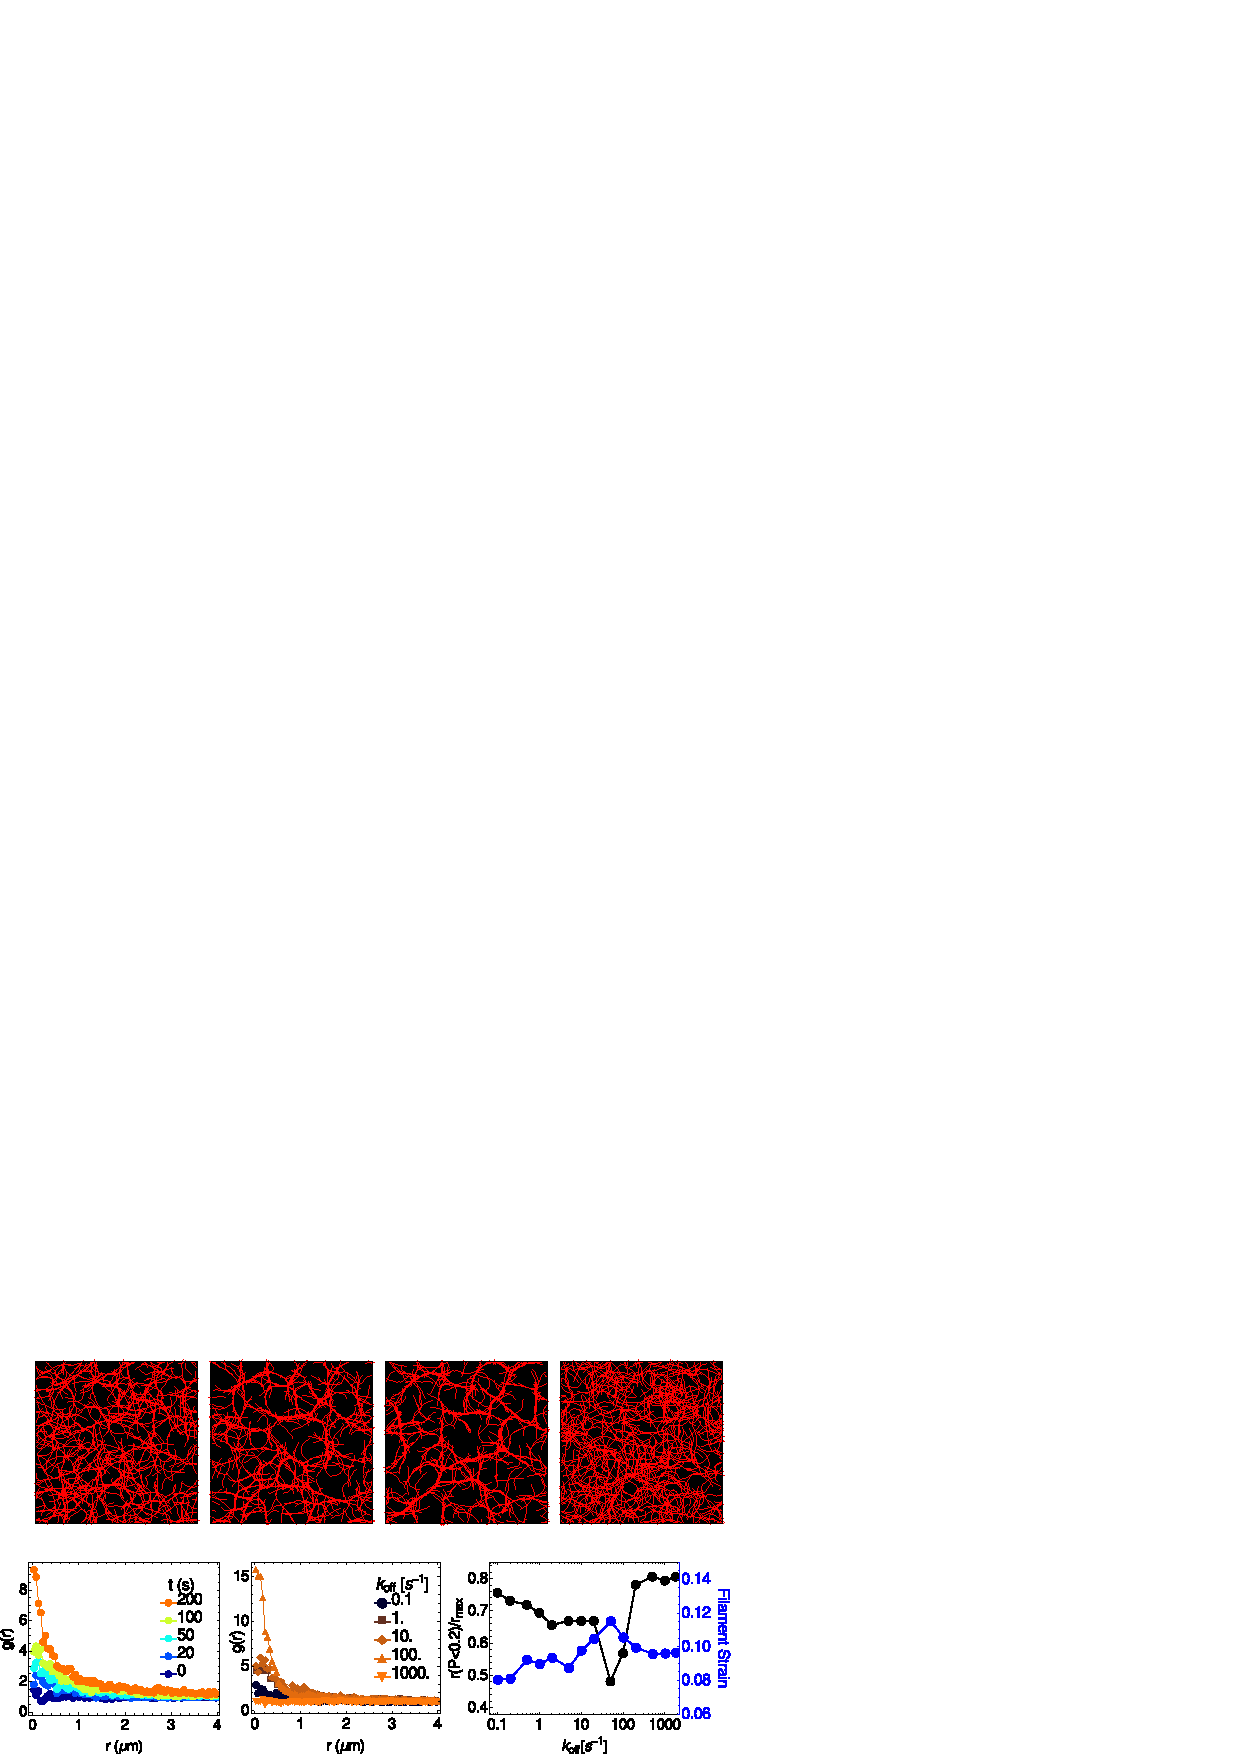
\includegraphics[width=\columnwidth]{figs/bundling/full_figure.pdf}
  \caption{%
  \label{fig:bundle}%
 {\bf Crosslinker unbinding rate controls bundling of filament networks in a biphasic manner.} (\textbf{A}) {\color{red}Network configuration at} $t=200s$ for varying disassociation constants of {\color{red}crosslinks (not shown)}. Filaments {\color{red}are shown} in red. 
  (\textbf{B}) Radial distrbiution function of beads on an actin filament for the $k_\text{cl}^\text{off}=20 s^{-1}$ at
  various times. As the simulation proceeds, the higher peak at lower $r$ values shows {\color{red}increase in} bundle {\color{red}thichkness}.
  (\textbf{C}) Radial distribution function of actin filaments at $t=200$s for varying $k_\text{cl}^\text{off}$. 
  The curves show non-monotonic
  behavior, as both high and low $k_\text{cl}^\text{off}$ have a shorter correlation {\color{red}length} than curves with mid-range
  $k_\text{cl}^\text{off}$.  
  (\textbf{D}) We {\color{red}quantify the} non-monotonicity by the distance at which $80\%$ of the area under the curves in 
  (B) are covered. Lower values mean longer correlation lengths, indicating a larger magnitude
of bundling. We also show that the difference in filament strain across these simulations is minimal, less than $0.025$, and shows no clear relationship with the radial distribution functions. 
{\color{blue}SB: Move this elsewhere - Contrast this with contracting networks in \Cref{fig:contract}, where where filament strain ranges from $0$ to $0.35$ and correlates with network divergence}.  
}
\end{figure}
\subsection*{Tunable elastic behavior of crosslinked filament networks}
\par
The {\color{red}mechanical} properties of cross-linked F-actin networks are generally {\color{red}inferred} using rheological {\color{red}measurements} {\color{red}(cite)}. In a {\color{red}typical rheology}
experiment, actin and crosslinker proteins are mixed {\color{red}to} form a crosslinked mesh, {\color{red}and then} sheared in a rheometer by a prestress $\sigma_0$. The prestressed network {\color{red}is} then {\color{red}subjected to} a sinusoidal differential stress of magnitude
$d\sigma\ll\sigma_0$. By measuring the resulting strain, one can calculate the
differential elastic modulus: $G(\sigma_0) = d\sigma/d\gamma$. 
In experiments using a stiff crosslinker, such as scruin, the dependence of the differential modulus on high prestress 
is $G\propto\sigma_0^{3/2}$, indicating that this shear stiffening is a direct result of the nonlinear {\color{red}force-extension relationship} of actin~\cite{gardel2004,lin2010}. Experiments using more compliant crosslinkers, such as filamin, have found a softer
stiffening response, $G\propto\sigma_0$, indicating that a significant amount of stress is {\color{red}mediated through} the crosslinkers,
and not the {\color{red}filaments}\cite{kasza2009}.
\par 
These results suggest that the {\color{red}strain} stiffening behavior of a crosslinked network can be tuned by varying the crosslinker
stiffness. To test this possibility, the configuration of filaments shown in \Cref{fig:t0} was reproduced with varying crosslinker stiffness $k_\text{cl}$. 
To inhibit network restructuring, the detachment rates of the crosslinkers was set to zero. An affine strain of $\delta\gamma=0.001$ was applied such that the horizontal position of every actin bead ($x_a$) was shifted {\color{red}according to:}
\begin{equation}
  x_a \rightarrow x_a + \delta\gamma \left( {y_a\over Y} \right)
  \label{eqn:sllod}
\end{equation} 
following the overdamped SLLOD {\color{blue}(what's that?)} equations of motion \cite{evans1984}. The periodic boundary was simulatenously shifted
following the Lees-Edwards convention \cite{allen}. The mesh was then allowed to relax for $t_\text{relax} =
0.001$s before the next step strain of $\delta\gamma$. This {\color{red}protocol} was {\color{red}continued} for $T_f=0.5$s, {\color{red}allowing} the total strain {\color{red}to reach a value}: $\gamma T_f/t_\text{relax}=0.5$. Increasing $t_\text{relax}$ did not significantly change the simulation results (\Cref{fig:tRelax10}).  
\par
The {\color{red}elastic behavior of the network} for each crosslinker stiffness was measured by calculating $w$, the strain energy density at each timestep
\begin{equation}
  w(t) = {1\over X Y}\left(\sum_f{ U_f}+\sum_\text{cl}{U_\text{cl}}\right)
  \label{eqn:sed}
\end{equation}
where $U_f$ is {\color{red}the mechanical energy of individual filaments} (Methods) and $U_\text{cl}$ {\color{red}defines} the potential energy of each cross link. {\color{red}By} averaging
over windows of size $t_\text{relax}$, {\color{red}we determine} $w(\gamma)$. \Cref{fig:stress} shows the results of these calculations for various values of
crosslinker stiffness, $k_\text{cl}$. By varying the ratio of filament to crosslinker stiffness, we were able to {\color{red}modulate} the scaling {\color{red}exponent of the} power law {\color{red}dependence} of strain energy {\color{red}on} the strain. For extremely low $k_\text{cl}$, {\color{red}the strain energy scaled linearly with strain}, $w\propto \gamma$, {\color{red}indicating that} the network {\color{red}showed} no resistance to shear: $G=d^2w/d\gamma^2=0$. While for high $k_\text{cl}$,
{\color{red}we observe a neo-hookean strain stiffening behavior,} $w\propto\gamma^4$ {\color{blue}(cite Yair Shokef \& Sam Safran, PRL 2012)}. Thus, one can tune the behavior of these networks from being liquid-like, with $w\propto\gamma$, through
the {\color{red}hookean} elastic regime of $w\propto\gamma^2$, as well as strain stiffening regimes of $w\propto\gamma^3$ and
$w\propto\gamma^{3.5}$, {\color{red}as} {\color{red}previously reported} in experiments\cite{gardel2004, kasza2009}. 
\begin{figure}[H]
  \centering
  \includegraphics[width=0.8\columnwidth]{figs/elasticity/shear_result.pdf}
  \caption{%
    \label{fig:stress}%
    {\bf Tunable strain stiffening in crosslinked filament networks}. (A) Snapshots of a strained network ($k_a=k_\text{cl}=1000$ {\color{blue}units?}) at $t=0.1$s, $t=0.25$s and $t=0.5$s. 
    Color indicates stretching energy on each link, with white being the lowest and red being the highest. 
    (B) The potential energy of the network as a function of time shown at different strains: $\gamma_0=0.1$ (circles) $\gamma_0=0.25$ (squares) and $\gamma_0=0.4$ (triangles) where $t_0=\gamma_0\times 1$s. Black dashed line shows the strain {\color{red}protocol}.  {\color{blue}SB: can we show a finer sampling of U?} 
    (C) Strain energy density ($w=U/$area) for various values of crosslinker stiffness $k_\text{cl}$. Blue dashed line
    indicates expected behavior for a {\color{red}linearly} elastic solid $w\propto \gamma^2$, and green dashed line indicates strain stiffening
    behavior of $w\propto \gamma^{3.5}$ as {\color{red}expected for semiflexible polymer networks} \cite{gardel2004,lin2010}.
   (D) Power law {\color{red}exponent} of $w(\gamma)$, evaluated via least squares fit to $\ln{\gamma}$ vs $\ln{w}$. {\color{blue}SB: could we annotate this plot marking the different phases - liquid-like, hookean solid, semi flexible polymer networks, neohookean behavior?}. 
  }
\end{figure}

\subsection*{{\color{blue}Cooperative} sorting of filament polarity by molecular motors}
{\color{red}Molecular} motors are modeled as {\color{red}active} crosslinkers {\color{red}such} that a bound head will processively {\color{red}walk} toward the barbed end of the filament {\color{red}with load dependent speed and kinetics} (see Methods for details). 
This implementation allows for {\color{red}active} filament sliding and filament buckling, as {\color{red}elucidated} in \Cref{fig:toys}, 
both of which are instrumental for actomyosin contractility \cite{murrell2012}.
In large networks, motors can translocate across filaments, {\color{red}induce filament buckling}, and {\color{red}also enhance} network connectivity\cite{murrell2014}. 
\begin{figure}[H]
  \centering
  \includegraphics[width=\textwidth]{figs/minimal.pdf}
  \caption{\label{fig:slide}
  \label{fig:toys}%
  {\bf Buckling, sorting and sliding of filaments by motors}. Time series of three antiparallel $10\ \mu$m filaments (red) interacting with a minimal set of motors (white) and crosslinkers ({\color{red}yellow}) for $10$ s. Barbed ends of filaments are marked in blue. {\color{blue}could we have a legend in the fig. for the different colors/entities?} 
  (A) Semiflexible filaments ($21$ bead-spring chain) pinned on the left by a crosslinker, so the motor-filament interaction yields contraction via buckling. 
  (B) Filaments are rigid ($2$-bead-spring chains) and unpinned, so motor-filament interaction yields {\color{red}unimpeded sliding of} filaments. {\color{red}As a result,} they transition from an initially extended state to a contracted state at $t=3$s, and back to a {\color{red}fully} extended and {\color{red}polarity sorted} state at $t=10$ s.
  (C) {\color{red}Filaments are} same as in (B), but with a population of crosslinkers near the filaments that {\color{red}arrests the filaments} in a contracted state. {\color{blue} Could we show the corresponding dipole moment vs time (although it may be obvious to us)?}} 
\end{figure}

To isolate the role of active motors on assemblies of semiflexible filaments, the actin assembly (\Cref{fig:t0}) was generated without  
crosslinkers at filament intersections, but with $0.5\ \mu$m {\color{red}long} motor minifilaments scattered uniformly throughout the simulation cell. 
In these simulations, the motor duty ratio was kept near unity to replicate the behavior of a myosin minifilament, 
while the density of motors was varied between {\color{red}the different} simulations. The results, shown in \Cref{fig:polarity_sorting}, indicate that at higher motor densities, filaments are sorted by polarity, but are
not clustered {\color{red}in space}. Motors aggregated on the barbed ends of filaments
and thereby brought the {\color{red}different} barbed ends together to form asters. The magnitude of polarity sorting is measured
by calculating the average distance of a bound motor from the barbed end of the filament to which it is bound. As seen from 
\Cref{fig:polarity_sorting} A-B, increasing motor density had the effect of decreasing this distance, indicating a larger
magnitude of polarity sorting. {\color{blue}how does the end-detachment rate of motors modulate this behavior?} It appears therefore that this form of {\color{red}polarity organization} and restructuring is highly tunable. {\color{blue}it seems this behavior is also highly cooperative}
\begin{figure}[H]
\centering
    \includegraphics[width=\columnwidth] {figs/polarity_sorting/ps_fig.pdf}
  \caption{%
  \label{fig:polarity_sorting}%
 {\bf Tunable polarity sorting in active networks.} (A)
  Network configurations after the completion of polarity organization ($t=96$ s). 
  Filaments {\color{red}are shown} in red and motors in white. A maximum of $1000$ motors are shown in each case.
 (B) {\color{red}Probability density} of the distance of an attached motor
   head from the barbed end of the filament to which it is attached for varying motor density (at $t=96$ s).
 (C) The average distance of a motor head from the barbed end as a function of motor density. {\color{blue} SB: Can we normalize the distance and plot the inverse quantity vs motor density? The behavior may look Hill-like such that you may extract a cooperatively coefficient by fitting the hill function. This will illustrate the cooperative polarity sorting behavior}
 (D) Radial distribution function for barbed ends shows a strong dependence on motor density. For $\rho_m=5\ \mu$m$^{-2}$, a {\color{red}prominent secondary} peak is visible at the motor rest length $l_m=0.5\ \mu$m.
 } 
 \end{figure}
\subsection*{Contractility emerges from a competition between filament bundling and polarity sorting}
\par
When both crosslinkers and motors are {\color{red}mixed} with semiflexible filaments, the assemblies {\color{red}behave} contractile. 
To {\color{red}elucidate} this behavior, actin filament assemblies were initialized (\Cref{fig:t0}) with crosslinkers 
at their intersections, and with motors scattered uniformly throughout the cell. The motor density was varied between simulations from $0.1-10\mu m^{-2}$.
The crosslinkers were kept sticky with a low duty ratio, while the motors were highly active
with a high duty ratio. This ensured that the connectivity of the network was almost exclusively controlled by crosslinkers while force generation was controlled by motors. {\color{blue}SB: thus, the decoupling between connectivity and force generation is by design. in reality, just motors are sufficient to yield contractility. need to discuss this}
\par
The results of these {\color{red}simulations and the final network configurations are given} in \Cref{fig:contract}A. The {\color{red}net} contractility was measured by
interpolating a velocity field from the displacement vectors of filament beads, and measuring the divergence of the
velocity fields~\cite{murrell2014}. A negative divergence indicates a net contractile {\color{red}behavior}. As evident from \Cref{fig:contract}(B), a higher motor density leads to larger contractility. \Cref{fig:contract}(D) shows
that actin buckling, here measured as the change in the end to end distance, $\Delta s$, of an actin filament:
\begin{equation}
  \Delta s = \left(1 - {|r_{N_B}-r_0|\over\sum_{i=1}^{N_B}{|r_i-r_{i-1}|}}\right) 
  \label{eqn:fil_strain}
\end{equation}
correlates with contractility, suggesting that the primary mechanism driving
contractility in these flexible networks is {\color{red}filament} buckling, as {\color{red}observed} in experiments \cite{murrell2012}. 
\begin{figure}[H]
  \centering
  \includegraphics[width=\columnwidth]{figs/divergence/div_fig.pdf}
  \caption{%
  \label{fig:contract}%
  {\bf Contractile behavior of assemblies of motors, filaments and crosslinks}. (A) 
  Network {\color{red}configurations} at their largest contractile {\color{red}strain} for different motor densities. Filaments {\color{red}are shown} in red and motors in white. Only $1000$ motors are shown in each case.
  (B) {\color{red}Spatially averaged} divergence {\color{red}of filament flow field} as a function of time for
  networks of varying motor density. Networks with a higher density of motors are more contractile. {\color{blue} Could we show the corresponding vector maps, overplayed on div heat map, for the configurations in panel A?}
  (C) Average filament strain (\Cref{eqn:fil_strain}) as a function of time for the same networks. 
  (D) Correlation between filament strain and the network strain, {\color{red}which is} measured 
{\color{red}by the} negative of divergence for all times, averaged over bins of size $0.005$, for all motor densities.
 } 
\end{figure}  

\subsection*{Modulating ensemble motor behavior}
While the force dependent attachment/detachment kinetics and speed of an individual myosin motor is {\color{red}a model input} (Methods), the ensemble behavior of many
motors could provide a benchmark that the simulation is {\color{red}capable of reproducing dynamics observed in actin motility}
assays {\color{blue}\cite{walcott2012} (cite Riveline et al Eur. Biophys. J. 1998)}. {\color{red}In a classical} motility assay experiment, a layer of myosin is
adhered to a plate and actin filaments are placed on top of the {\color{red}motors}. Because the myosin cannot diffuse, they instead
slide the actin filament across the assay.
Although this experiment typically involves single myosin heads, and not myosin minifilaments, we believe that
functionally the situations would be equivalent, with the substitution that each model motor head approximates the
activity of dozens of single molecule myosin heads. 
{\color{red}Previous experiments} \cite{harris1993, umemoto1990} {\color{red}have reported} a nonlinear dependence of the speed of an 
actin filament on the concentration of myosin, the length of
the actin filament, and the concentration of ATP in the sample. By allowing filaments to interact with {\color{red}a group of} motors, one
can monotonically increase the filament speed to a {\color{red}constant value}. 
\par
To explore {\color{red}the dynamics of} this {\color{red}assay}, we randomly distributed motors on a $50\ \mu$m $\times 50\ \mu$m periodic simulation cell and
{\color{red}tethered} one head of each motor to {\color{red}a solid surface}. Filaments were {\color{red}then introduced} in the simulation cell and 
allowed to interact with the {\color{red}free} motor heads. The {\color{red}strength} of motor-filament interactions was manipulated by varying the motor concentration $\rho_m$, the filament contour length $L$, and the duty ratio $r_D =
k_m^\text{on}/(k_m^\text{on}+k_m^\text{off})$. 
The results are shown in \Cref{fig:motility}, where we have used the dimensionless {\color{red}control} parameter $\mathcal{M}=\rho_m L^2 r_D$, {\color{red}representing the average number of bound motor heads,} to {\color{red}tune filament motility}. 
\par
{\color{red}Our} findings are qualitatively similar to the {\color{red}previously reported} experimental results. 
{\color{red}At low $\mathcal{M}$, i.e.} low motor density, filament length and duty ratio, transverse filament fluctuations dominate over longitudinal motion as the filament is not being propelled by motors faster than diffusion ({\color{red}\Cref{fig:motility}(B)}). However, as {\color{red}$\mathcal{M}$ is} increased, longitudinal
motion dominates. This can be {\color{red}inferred} from the {\color{red}dependence of the} mean squared displacement, plotted in \Cref{fig:motility}(D), where low $\mathcal{M}$ 
yields diffusive behavior with $\langle r^2 \rangle \propto t$, and the motion becomes ballistic with $\langle r^2\rangle\propto t^2$ 
as $\mathcal{M}$ {\color{red}approaches 100}.
The {\color{red}longitudinal} speed of {\color{red}the filament} plateaus at $v_{||}\approx 1\mu$m/s, which is the average unloaded {\color{red}speed of a single motor head} {\color{blue}(cite)}. \Cref{fig:motility}(C) shows that aside from being propelled, filaments are also
buckled in the presence of a large number of motors, as the filament strain increases with increasing $\mathcal{M}$. 
Although there are no explicit crosslinkers, at a high enough concentration, motors near the barbed end 
of a filament will pin the filaments for a short time, and induce buckling the same way as crosslinkers 
do in contractile networks. {\color{blue}( we should definitely cite Schaller et al Nature 2010)}
\begin{figure}[H] 
    \centering
    \includegraphics[width=\columnwidth]{figs/motility/mot_fig.pdf}
  \caption{%
  \label{fig:motility}%
  {\bf Active transport by a collection of motors}. (A) Position of a filament for $\rho_m = 10\ \mu$m$^{-2}$ and $L = 16\ \mu$m for
  different values of the duty ratio. White filament is {\color{red}the configuration at} $t=0$ and dark red {\color{red}represents} $t=90s$. {\color{blue}can we have a colorbar showing in time in the figures?} Blue dot marks the barbed end of filaments.  
  (B) Longitudinal filament speed (circles) monotonically increases to a plateau while transverse speed 
  (squares) decreases with larger motor density, filament length, and duty ratio. Green: $\rho$ variable, $L=15\ \mu$m,
  $r_D=0.95$; Red: $L$ variable, $\rho_m=4\ \mu$m$^{-2}$, $r_D=0.95$; Blue: $r_D$ variable, $\rho_m = 10\ \mu$m$^{-2}$, $L=15\ \mu$m.  
  (C) Filament strain, defined in \Cref{eqn:fil_strain}, as a function of the dimensionless
  parameter $\mathcal{M}=\rho_m L^2 r_D$, indicating that {\color{red}filament} is being buckled {\color{red}during propulsion} by motors. 
  (D) Mean squared displacement for various values of $\mathcal{M}$ shows that the transition from
  diffusive (blue dashed line) to ballistic (red dashed line) behavior occurs at low values of this parameter.     
 }
\end{figure}
%%%%%%%%%%%%%%%DISCUSSSION%%%%%%%%%%%%%%%%%%%%%

\section*{Discussion}
{\color{blue} I feel the discussion is a bit too long and can be focused more based on the results section. Some detailed discussion on prior modeling work could relegated to the supplement while describing method details.}\\
The goal of this paper is to introduce a framework that could accurately and efficiently simulate active 
networks of {\color{red}filaments, motors}, and crosslinker proteins {\color{red}and predict} the various structural {\color{red}and mechanical} phases 
{\color{red}of the system}. In doing so, we have shown that our model can reproduce the key results of 
canonical {\color{red}{\it in vitro}} experiments {\color{red}involving F-actin, myosin and crosslinks}. {\color{red}We show that our} simulated networks {\color{red}exhibit tunable} strain stiffening {\color{red}upon shear}, and networks with dynamic crosslinkers
form bundles {\color{red}depending on turnover rate}. In simulated {\color{red}actin} motility assays, the filament speed scaled with motor density matched as observed experimentally, and networks with motors and crosslinkers robustly contracted. 
We have also expanded significantly on these experiments {\color{blue}(??)}. 

\par
For crosslinked networks, we show that the scaling of strain stiffening can be tuned by 
changing the crosslinker stiffness. Many other models have successfully {\color{red}explained} the 
viscoelastic properties of crosslinked actin networks \cite{mackintosh1995, head2003, wilhelm2003, kim2009}.  
For example, Head et al. {\color{red}performed simulations} with straight rod filaments with bending potentials at rod intersections, and was able to identify three {\color{red}distinct} elastic regimes,
characterized by the mean distance between crosslinkers and the temperature \cite{head2003}. Similar models used non-Hookean crosslinkers to show how unfolding can yield strain softening at large strain \cite{didonna2007}. Others 3D models, with explicit filament bending have examined the frequency dependence of these networks and reproduced theoretical predictions\cite{gittes1998,kim2009,muller2014}.
{\color{red}Here} we have shown that by modeling crosslinkers as idealized Hookean springs, 
and {\color{red}by} varying their stiffness, one can modulate the {\color{red}mechanical properties of the network by tuning it from liquid-like material to strain-stiffening elastic materials}. 
This is particularly interesting, given that recent experimental findings suggest that one can engineer 
actin binding proteins of varying stiffness\cite{vieregg2016}.  

\par
The ensemble motion of many myosin motors with respect to a single actin filament has also been 
studied via simulation, in order to develop a realistic model of a myosin minifilament.
Erdmann and Schwarz, who used Monte Carlo simulations to verify a master equation that expresses 
the probability that $N$ motors are bound at time $t$ to a single filament\cite{erdmann2012} were able to make 
accurate predictions for the duty ratio and force velocity curves for myosin minifilaments. 
Stam et al. used simulations to study force buildup on a single filament by a multi-headed motor and found
distinct timescale regimes over which different {\color{red}molecular} motors could exert force and act as crosslinkers
\cite{stam2015}. These models of actin-myosin interaction are important to understand the mechanics at
the level of a single filament, and their results can be incorporated into larger network simulations.
However, our results show that even a minimal model of actin and myosin is able to capture the ballistic and
longitudinally processive behavior of actin filaments in a {\color{red}canonical} motility assay experiment.

\par
Other actomyosin models have explored the driving mechanisms behind contractility. 
Dasanyake, et. al., extended the model in \cite{head2003} to include a term in the potential energy that corresponded to
myosin motor activity, and observed the emergence of force chains that transmit stress throughout 
the network\cite{dasanyake2011}. 
Wang and Wolynes \cite{wang2012} model the F-actin networks as a graph of crosslinkers (nodes) and rigid actin filaments
(edges) in which myosin motor activity is simulated via antisymmetric kicks along the filaments and predict a
binary phase diagram of networks which are either contractile or not as a function of cross linker and myosin
densities. While the simplicity of these models is intriguing, they do not account for explicit filament buckling, 
and their integration is performed via Monte Carlo, more applicable to structure formation than dynamics.
We have shown that using an agent based model we can reproduce the experimentally observed contractility of actomyosin networks, 
that it scales with motor density, and that it correlates with filament buckling, both of which have been confirmed in in
vitro reconstitutions \cite{murrell2012,murrell2014}.

\par
Contractility and structure formation has also been explored in the context of agent based models. 
Nedelec used dynamic simulations of ensembles of filaments and motor proteins
to explore aster formation in microtubule-kinesin assemblies, as well as motility and contractility in actomyosin
\cite{nedelec2002,nedelec2007,ennomani2016}. 
Kim used an agent based approach of filaments, motors and crosslinkers, to explore a variety of topics, 
including bundling in crosslinked networks and force generation by myosin motors\cite{kim2009b, kim2014}. {\color{blue} (SB: we need to discuss this as i don't completely trust kim's simulations based on prior and ongoing correspondences.)}
While the bundling observed in \cite{kim2009b} was the result of crosslinkers that explicitly bind parallel filaments, 
we have that generic crosslinking leads to network coarsening and that this bundling effect depends strongly, 
and non-monotonically on the crosslinker-filament affinity. These bundled networks have the important physical property of being 
able to transmit forces large distances, and are thought to serve the biomechanical functionality 
of forming force chains to propagate stress throughout the cell. 

\par
Additionally, we showed that we can tune polarity sorting in filament assemblies. 
Polarity sorted networks can be used to by load-carrying motors to 
transmit cellular goods large distances, so insight into how a cell modulates this behavior could be extremely
helpful in biophysics and active matter. While this polarity sorting is similar to the aster formation seen in
\cite{nedelec2002,gordon2012}, we have shown that the process will also occur when filaments are semiflexible, 
have developed a reliable order parameter for measuring this process, and shown that the magnitude of this parameter increases
monotonically with motor density. 

\par
While our model is thorough in what it aims to simulate it is limited by a few experimental observations that are
currently not implemented. First, the structure of myosin minifilaments is significantly more complex than a two headed
spring. As mentioned, these minifilaments have dozens of heads, which allows them to walk along multiple filaments and
could result in subdiffusive behavior \cite{scholz2016} and significantly increase local network elasticity
\cite{murrellTalk}.
Another limitation of our system is that the actin filaments are static, and will not polymerize, depolymerize or
sever. Within actomyosin assays it is clear that recycling of actin monomers and to a lesser degree, filament severing 
plays an important role in contraction\cite{murrell2012}. Within the cytoskeleton, actin treadmilling is also important
for shape production. Additionally, these simulations are all run in $2D$ and without steric interactions, and
dimensionality and volume exclusion may play important roles. 
While we intend to address and investigate these limitations in future works, we believe that the successful
benchmarking of the simulation at various levels is a significant argument in favor of the current setup.

\par 
There are many unanswered questions regarding {\color{red}self-organization in} actomyosin networks that {\color{red}can be}
addressed using {\color{red}our} simulation, such as how {\color{red}actomyosin} controls the shape of cell membranes, {\color{blue}and they form force
propogating chains across the cytoskeleton - are there experiments showing this??)}. 
In particular, it is significantly easier to measure local forces and energies in simulation than in experiment ({\color{blue}forces can be measured in traction force experiments - however simulations can separately predict internal active forces}), 
so we expect this model will aid the process of isolating the particular mechanisms involved in restructuring these
polymer assemblies. We stress, however, that
the applicability of such a simulation package reaches beyond studying the phases of actomyosin networks.  
We believe this simulation can shed light on {\color{red}the mechanics and dynamics of} a variety of active polymer assemblies.
\par
Similar networks that involve other proteins also exist in the
cytoskeleton, such as microtubule-kinesin-dynein networks and could be investigated using this simulation methodology. 
Furthermore, the cytoskeleton demonstrates how populations of simple machines can self assemble into active materials with
useful mechanical properties, and one can use this simulation to efficiently design these types of self assembled
materials. Thus, the non-equilibrium molecular dynamics framework of this simulation can be used to model and study
many open questions in active matter and biophysics.

\section*{Methods}  
{\color{blue}SB: Could we split the methods section between the main paper and the supplement? I'd suggest minimizing details in the main methods and move the rest to the supplement.}
\paragraph{{\bf Actin Filaments.}} Actin filaments are treated as a worm-like chain, with each filament represented as a set of $N+1$ beads connected by $N$ harmonic springs (links), with an additional harmonic angular potential applied on the $N-1$ angles along the chain, as depicted in \Cref{fig:filament}(A). The linear springs 
penalize stretching of individual subunits and the $N-1$ angular harmonic springs penalize bending and enforce the length scale over which the filaments are semi-flexible. 

The internal forces on actin filaments can be obtained from the gradient of the potential energy $U_f$
\begin{eqnarray}
  U_f &=& U_{stretch} + U_{bend}\\
  U_{stretch}&=&{k_a\over2}\sum_{i=1}^{N}{(|d_i| - l_a)^2}\\\nonumber
  U_{bend}&=&{\kappa_B\over 2l_a}\sum_{i=2}^N{\theta_i^2}\\\nonumber
  \label{eqn:Ufil}
\end{eqnarray}
where $d_i = r_i-r_{i-1}$, $\theta_i = \arccos{\left({d_i\cdot d_{i-1}\over |d_i||d_{i-1}|}\right)}$, $k_a$ is the
stretching force constant, $\kappa_B$ is the bending modulus, and $l_a$ is the equilibrium length of a
link. 
\par
For a confined semiflexible filament, it has been show that for a polymer of a given persistence length $L_p$, the shortest length that should be considered as unbending ($l_a$) is given by $l_a\approx A^{2/3}L_p^{1/3}$ where $A$ is a length scale associated with the confinement of the
filament \cite{odijk1983}. In these simulations, filaments were confined by nearby motors and crosslinkers. Since the smallest motor or crosslinker density used was $\rho_m=0.1\mu m^{-2}$, $A\ge1/\sqrt{0.1\mu m^{-2}}\Rightarrow l_a\ge5\mu m$. In general, we used $l_a=1\mu m$.
The bending force constant is derived from the persistence length $L_p$ such that
$\kappa_B = L_p k_B T$ where $k_B$ is Boltzmann's constant and $T$ is the temperature \cite{rubinstein}. Experimentally,
the stretching force constant has been measured to be in the approximate range $k_a=40-70pN/nm$ \cite{kojima1994, higuchi1995}; however, simulating a
network of filaments with this large of a stiffness is computationally inefficient since the maximum timestep of a simulation is inversely proportional to the largest stiffness in the simulation. Therefore, we chose ${\kappa_B\over l_a} <<k_a$, so that the filaments were still much easier to bend than to stretch, enabling us to run simulations of experimentally relevant dimension. We show that our simple filament model exhibits expected behavior for a semiflexible filament in the next section and we have further verified that $k_a$ did not effect the persistence length of the filament, as seen in \Cref{fig:wlc_supp}. 
\par
Since actin bending is instrumental for actomyosin contraction, and simulating precise bending moduli is non-trivial, we tested our filaments by measuring spatial and temporal fluctuations and comparing with theoretical predictions.
In a two dimensional WLC, a bending of two adjacent segments is expected to result in a local change in free energy of ${\kappa_B\over2l_a\theta_i^2}$, and it is predicted that \cite{frontali1979}
\begin{equation}
  \langle\theta^2(l)\rangle = {l\over L_p}
  \label{eqn:thsq}
\end{equation}
\begin{equation} 
  \langle\cos(\theta(l))\rangle = \exp{(-l/2L_p)}
  \label{eqn:costh}
\end{equation} 
where $\theta(l) = \theta_j - \theta_i$ where $1<i<j\le N$, $l = l_a(j-i)$ and $L_p$ is the persistence length. To test our model against these equations, we simulate $100$ filaments of $L=200\mu m$ and $\kappa_B=0.08 pN\mu m^2$ at $T=300K$ for $T_f = 100s$ and measured the resulting filament configuration every $1s$. We discard the first $10$ seconds of each simulation to allow equilibration, and we used only the middle $150 \mu m$ of the filament to calculate these correlation functions.
%For each of the $90000$ filament configurations, and for each $l\in{0,1,2,..,150}\mu m$,
%$\theta^2(l)$ and $\cos(\theta(l))$ were calculated, and their respective averages are plotted in 
%\Cref{fig:avgTh}, along with the expected behavior given the input $\kappa_B$.  
\Cref{fig:kb} shows that the measured persistence length, obtained by performing a least squares fit to plots of $\log{(\langle cos(\theta(l))\rangle )} $ for various values of $\kappa_B$ yields the expected result over at least $3$ orders of magnitude. Further measurements of the persistence length as well as verifications of its independence on other filament parameters is available in the supplement \Cref{lpCalc}.
\par
An additional prediction for semiflexible filaments is the scaling of fluctuations with time. 
Fluctuations transverse to the filament orientation have been 
shown to increase as a function of time as $\langle dr_{\perp}^2\rangle\propto t^{3/4}$ while longitudinal fluctuations have been shown to follow the power law
$\langle dr_{||}^2\rangle\propto t^{7/8}$ \cite{everaers1999}. To tests these predictions, we followed the procedure outlined in
\cite{everaers1999} and generated $N = 100$ initial filament configurations of a $20\mu m$ filament. For each configuration we ran $M = 100$ simulations of the filament fluctuating for $1s$. At each time step we collected the $2N$ positions of the filament ends, $r_e(t)$. We then calculated the eigenvalues of the covariance matrix $cov(r_e(t)\cdot \hat{i},r_e(t)\cdot \hat{j})$ where
$i,j\in\{x,y\}$.
The larger eigenvalue $\lambda_1(t)$ corresponds to the slower longitudinal fluctuations
(i.e., $\lambda_1(t)\propto t^{7/8}$) while the smaller eigenvalue corresponded to the faster perpendicular fluctuations
($\lambda_2(t)\propto t^{3/4}$). We show  in \Cref{fig:filament}(C) that the our simulation exhibits scaling of these eigenvalues in good agreement with the prediction of Ref. \cite{everaers1999}.
\begin{figure}[H] 
  \centering
   \includegraphics[scale=1]{figs/filament/pl_fig.pdf}
  \caption{\label{fig:filament}
 (A) Sketch of semiflexible filaments (red); motors (green) binding, unbinding, and walking; and crosslinkers (blue) connecting filament intersections. Zoom in of the filament model shows a segment of the bead spring chain, identifying the angle used in \Cref{eqn:Ufil}.
  (B) Decorrelation of tangent vectors (red dots) and fluctuations in angles between links (blue dots) 
  as a function of the arc length between them. Red dashed
  line is $e^{-s/2L_p}$ shows the expected behavior from the input bending modulus of $0.08 pN-\mu m^2$ and blue
  dashed line has slope $1/L_p$.
  (C) Eigenvalues of covariance matrices for the positions of endpoints of filaments as a function of time. We analyze fluctuations of $N=100$ filaments, with each point the average over the $2N$ eigenvalues for $\lambda_1(t)$ and $\lambda_2(t)$ and error bars showing the standard deviations for the
distribution of these values. Blue
  dots shows the longitudinal fluctuations and the red dots shows the transverse fluctuations. Red dashed line is
  $t^{3/4}$ and blue dashed line is $t^{7/8}$ as predicted by \cite{everaers1999}. 
}
\end{figure} 
\paragraph{{\bf Crosslinkers.}}
Crosslinker proteins dynamically connect actin filaments, thereby propogating force from one to
another. Thus model crosslinkers, must be able to attach and detach from actin filaments,
and be compliant in order to propagate force. They are therefore modeled as hookean springs, with stiffness
$k_\text{cl}$ and rest length $l_{cl}$. Like actin filaments, the Young's modulus of
most crosslinkers is significantly higher than would be reasonable to simulate; therefore we set $k_\text{cl} = 1-100pN/\mu m$ was
so that the bending mode of actin filaments was signicantly softer than the stretching mode of
crosslinkers. Their rest length $l_{cl}$ differs by the type of cross-linker and ranges from $~10 nm$ for fascin to $150 nm$
for filamin. 
\par
At each time step of the simulation an unattached crosslinker head is allowed to attach to nearby
filaments and an attached crosslinker head can detach. 
The probability of a head attaching to an actin filament is a Gaussian distributed random variable, such that
\begin{equation}
  P_{cl}^{on} = k_\text{cl}^{on}dt\exp(-r^2/R^2)
  \label{eqn:cl_on}
\end{equation} 
where $r$ is the shortest distance from the head to the actin filament and $R = \sqrt{2k_B T\over k_\text{cl}}$ 
where $k_B$ is Boltzmann's constant and $T$ is the temperature. 
For crosslinker detachment we assume that the behavior is that of a slip bond, such that a higher
tensile force along the crosslinker backbone will result in a higher probability of detachment. Thus, 
\begin{equation}
  P_{cl}^{off} = k_\text{cl}^{off} dt\exp{\left(  F x_{cl}/k_B T\right)}  
  \label{eqn:cl_off}
\end{equation}
where $F$ is the force along the crosslinker backbone, and $x_{cl}$ is a characteristic bond length \cite{stam2015}. 
\par
When a crosslinker is bound to a filaments at both ends, it will necessarily be stretched or compressed. 
If it were allowed to relax independently of the actin filaments to which it is bound. 
it would no longer lie on those filaments. Therefore, the tensile force stored on a stretched or compressed
crosslinker is propagated onto those actin filaments via the lever rule outlined in 
\cite{nedelec2002, gordon2012}. Thus, if the tensile force of a motor at point $r_j$ between filament beads $i$ and $i+1$ is
$F_{cl}$, then, 
\begin{eqnarray} 
  F_i &=& F_{cl}\left|\left( {r_j - r_i \over r_{i+1} - r_i }\right)\right|\\\nonumber
  F_{i+1} &=& F-F_i 
  \label{eqn:lever}
\end{eqnarray}
will be the forces on beads $i$ and $i+1$ respectively due to the crosslinker.
\paragraph{{\bf Motors.}}%\label{sec:methods_motors}
Within the cytoskeleton, tens of myosin II motors aggregate into bipolar ensembles called myosin minifilaments
\cite{stam2015}. While the mechanochemical process through which individual myosin motors walk along actin filaments is complex, 
motility assay experiments have shown that on average bound myosin II heads walk at an unloaded speed of $v_0\approx1\mu m/s$ along actin
filaments\cite{finer1994}. To a first approximation, minifilaments therefore should also 
have a mean speed of $1\mu m/s$ (although see \cite{stam2015} and \cite{walcott2012} for higher order measurements). 
Since myosin also functions to increase the local elasticity of networks wherever it is bound, the myosin is modeled
similarly to a crosslinker, in that it behaves like a hookean spring with two heads, a stiffness $k_{m}$ and a rest
length $l_m$. It should be noted, however, that the two heads of this spring do not correspond directly to individual
molecular myosin heads; rather each of them represents tens of myosin molecules, and their rate constants will reflect
that notion. 
It would be undesirable for a myosin minifilament to stretch, 
since experimentally they have a very high
Young's modulus and it is unlikely that their length would change noticably in the cytoskeleton. Thus we set $k_m\gg\kappa_B/l_a$
so that the bending of actin is still the softest mode. 
The rest length was set to the average length of minifilaments \cite{niederman1975}.
Attachment and detachment kinetics for motors are the same as for crosslinkers, subscripted with $m$
instead of $cl$ in \Cref{eqn:cl_on,eqn:cl_off}. One extra parameter is needed $k_m^{end}$ for the
detachment of myosin from the barbed end of a filament, as detachment from the end is significantly more probable than
from the rest of the filament.
Similarly, force propogation onto minifilaments is done using the lever rule described in \Cref{eqn:lever}.
\par
Unlike crosslinkers, motors process towards the barbed end of actin filaments to which they are bound 
at speeds that vary depending on the tensile force along the crosslinker. 
The relationship between motor velocity and tensile force is modeled linearly, such that the motor head 
will speed up if the minifilament is
compressed (pre-powerstroke) and slow down if the minifilament is stretched (post powerstroke) going to
$0$ when the force on the minifilament is the stall force $F_s\approx 3.85pN$ \cite{nedelec2002, gordon2012}; i.e.,  
\begin{equation} 
  v(F_{||}) = v_0\left( 1-{F_{||}\over F_s}) \right)
    \label{eqn:myo_vel}
\end{equation} 
where $F_{||}$ is the force on the motor, projected along the tangent vector of the
actin filaments.
The minor differences between crosslinkers and motors allow us treat them equivalently, by 
setting $v_0 = 0$ for the crosslinkers.  

\paragraph{{\bf Dynamics.}} We use Langevin dynamics to solve for the motion of actin filaments, myosin minifilaments and crosslinkers.
The Langevin equations of motion for a spherical bead of
mass $m$ and radius $R$ at position $r(t)$ at time $t$ can be written,
\begin{equation}
  m\ddot{r}(t) = F(t) + B(t) - 4\pi R\nu \dot{r}(t)
  \label{eqn:lang}
\end{equation} 
where $F(t)$ is the force on the particle due to its interactions and $B(t)$ is Brownian forcing term, to simulate a temperature, $\nu$ is the dynamic viscosity of the bead's
environment, and we have used the Einstein relation for the damping term.  
Since the fastest motion in this simulation is that of the myosin, and a $0.4\mu m$ myosin minifilament moving at
a speed of $1\mu m/s$ in a liquid at least as viscous as water ($\nu_D=10^6\mu m^2/s$ dynamic viscosity) has a very low Reynold's
number ($Re \approx 4*10^{-7}$) we can treat the dynamics in the overdamped limit where the equation of motion is \Cref{eqn:lang} without the acceleration term, i.e. with $m=0$.
Furthermore, in the limit of small $\Delta t$, we may write $\dot{r(t)} \approx {r(t+\Delta t)-r(t)\over \Delta t}$. These two
approximations allow us to rewrite \Cref{eqn:lang} as 
\begin{equation}  
  r(t+\Delta t) = r(t) + F(t)\mu \Delta t + B(t) \mu \Delta t
\label{eqn:overdamped}
\end{equation}
where $\mu = (4\pi R\nu)^{-1}$. For the Brownian term, we use the form of Leimkuhler and Matthews \cite{leimkuhler2012,leimkuhler2013} that has
been shown to minimize deviations from canonical averages in harmonic systems,
\begin{equation}
  B(t)=\sqrt{2k_BT\over\mu \Delta t}\left({W(t)+W(t-\Delta t)\over2}\right)
  \label{eqn:baoab_brownian}
\end{equation} 
where $W(t)$ is a Wiener process, in this case a random number drawn from the normal distribution with mean zero and standard deviation of unity.

\paragraph{{\bf Environment.}} Because the probability of motor attachment decays as a Gaussian function of distance from the filament, it would be highly inefficient to attempt motor attachments with every filament in the simulation.  Rather, we choose to test for connections only within a cutoff distance
$r_c>3R/2$ (where $R$ is defined above as in \Cref{eqn:cl_on}). A grid of lattice size $2r_c$ is drawn in the $2D$ plane of the simulation, and the position of a filament is approximated as the points on the grid nearest to the beads of the filament. Thus, to determine if a motor will bind to a filament at time $t$, it is sufficient to only attempt attachment to filaments that are indexed at the four nearest grid points to a motor. 
\par
In general, we use periodic boundary conditions so as to limit effects of a boundary and to mimic a system larger than the one we simulate. Lees-Edwards boundaries \cite{allen} were used for shearing simulations, and hard wall boundaries have also been implemented.
The value for $\Delta t$ in \Cref{eqn:overdamped} generally depends on both the unloaded myosin speed
$v_0$ and the largest stiffness in the simulation $k_f$. For $k_f = 10pN/\mu m$ and $v_0=1\mu m/s$ a value of $\Delta t = 0.00001 s$ was sufficiently low to solve \Cref{eqn:overdamped} for hundreds of seconds without spuriously generating configurations of very large energy.
The length and width of the simulations were chosen so as to be high enough to avoid boundary artifacts. 
A complete list of simulation parameters used throughout this article is provided in {\color{red}Supplementary} \Cref{tab:params}. {\color{blue}make the Table supplementary?}
\begin{table}
  \caption{List of Parameter Values}
  \centering
  \begin{tabular}{|C{1cm}|L{6cm}|C{2cm}|C{2cm}|C{2cm}|C{2cm}|}
    \hline\hline
    Symbol & Description (units) [ref] & $L_p$ & Shear & Motility Assay & Networks\\
    \hline
    &\bf{Actin Filaments}& & & &\\
    \hline
    $N_B$ & Number of beads & $21-201$ & $16$ & $16$ &$16$\\
    $l_a$ & Link Rest Length ($\mu m$)\cite{odijk1983}& $1$ & $1$ &$1$& $1$\\
    $k_a$ & Stretching Force Constant ($pN/\mu m$) & $0.01-10$ & $10$ & $1$ & $1$\\
    $\kappa_B$ & Bending Modulus ($pN\mu m^2$)\cite{ott1993} & $0.002-5 $ & $0.08$ & $0.08$ & $0.08$\\
    \hline
    &\bf{Myosin Minifilaments}& & \\
    \hline
    $l_m$ & Rest Length ($\mu m$)\cite{niederman1975} & n/a & n/a & 0.5 & 0.5\\
    $k_m$ & Stiffness ($pN/\mu m$)& n/a & n/a & $1$ & $1$\\
    $k^{on}_m$ & Attachment rate at distance $r=0$ ($s^{-1}$)& n/a & n/a &$2-4000$ &$3600$\\
    $k^{off}_m$ & Unloaded head detachment rate ($s^{-1}$)& n/a & n/a & $200$ &$200$\\
    $k^{end}_m$ & Unloaded head detachment rate at the barbed end of the filament ($s^{-1}$)& n/a & n/a &$2000$ &$2000$\\
    $x_m$ & characteristic bond length ($\mu m$) \cite{stam2015}& n/a & n/a & $0.0004$& $0.0004$\\
    $v_0$ & Unloaded speed ($\mu m/s$) \cite{kron1986}&  n/a & n/a & $1$ & $1$\\
    $F_s$ & Stall force of myosin ($pN$)\cite{veigel2003}& n/a & n/a & $3.85$ & $3.85$\\
    \hline
    &\bf{Crosslinkers} & & \\
    \hline
    $l_{cl}$& Rest Length (Filamin) ($\mu m$)\cite{ferrer2008} & n/a &$0.150$ &n/a&$0.150$ \\
    $k_\text{cl}$ & Stiffness ($pN/\mu m$)& n/a & $1,10$ & n/a& $1$\\
    $k^{on}_{cl}$ & Attachment rate at distance $r=0$ ($s^{-1}$)& n/a & $10^6,10^5$ &n/a &$3600$\\
    $k^{off}_{cl}$ & Unloaded head detachment rate ($s^{-1}$)& n/a & 0 & n/a&$0.2$\\
    $x_{cl}$& characteristic bond length ($\mu m$) & n/a & $0.0004$ & $0.0004$ & $0.0004$ \\
    \hline
    &\bf{Environment} & & \\
    \hline
    $dt$ & Dynamics timestep (s) & $10^{-4}$ & $10^{-6},10^{-5}$ &$2.5\times10^{-4}$ &$2.5\times10^{-4}$ \\
    $T_F$& total simulated time (s) & $100$ & $0.5$ & $100$ & $500$ \\
    $X$, $Y$ & Length and width of assay ($\mu m$)& n/a & $75$ & $50$ & $75$\\
    $r_c$ & Mesh (actomyosin binding site) size ($\mu m$) & $n/a$ & $0.2 $ & $0.2 $& $0.2 $ \\ 
    $T$ & $k_B$ * Temperature ($pN\mu m$)& $0.004$ & $0.004$& $0.004$& $0.004$\\
    $\nu$ & Dynamic viscosity ($mg/(\mu m s)$) & $0.001$& $0.001$& $0.001$& $0.001$\\
    $\gamma$ & Strain (\%) \cite{stricker2010}& n/a& $0.001$&n/a&n/a\\
    $t_\text{relax}$ & Amount of time between sequential strains (s)& n/a& $0.001$ &n/a&n/a\\
    \hline
  \end{tabular}
  \label{tab:params}
\end{table}



\section*{Acknowledgements}  
We thank M. Gardel, J. Weare, C. Matthews, F. Nedelec, F. Mackintosh, and M. Murrell for helpful discussions. This research was supported in part by the University of Chicago Materials Research Science and Engineering Center (NSF Grant No. 1420709). S.L.F. was supported by the Department of Defense (DoD) through the National Defense Science \& Engineering Graduate Fellowship (NDSEG) Program. G.M.H. was supported by an NIH Ruth L. Kirschstein NRSA award (1F32GM113415-01).
\bibliography{actosim}
\bibliographystyle{unsrt}

\beginsupplement
\section{Supplement}
\subsection{Algorithm Pseudocode}
In pseudocode we can describe each timestep of the simulation as follows
\begin{verbatim}
For Each Bead on Each Filament:
    Update force from filament stretching
    Update force from filament bending\end{verbatim}
\verb|    Update position via | \Cref{eqn:overdamped}\begin{verbatim}
For Each Head on each Motor (cross-linker)
    If head is unattached
        try to attach
        Add up forces (stretching)\end{verbatim}
\verb|    Update position via | \Cref{eqn:overdamped}\begin{verbatim}
    If head is attached\end{verbatim}
\verb|        Update position via | \Cref{eqn:overdamped}\begin{verbatim}
        Try to detach
        If not detached 
            Step toward barbed end
            Update attached actin with stretch force
Update neighbor lists
\end{verbatim}
\subsection{ Further tests of the WLC model }\label{lpCalc}
From \Cref{eqn:costh} the distribution of the square of end to end distances can be calculated as 
\begin{equation}
  \langle r^2\rangle=\int_0^L{ds'}\int_0^L{ds \exp{(|s-s'|)/(2L_p)}}=4L_p L\left( 1-{2L_p\over L}\left( 1-\exp{(-L/2L_p)} \right) \right)
  \label{eqn:r2}
\end{equation} 
Thus, \Cref{eqn:r2} provides a third method for measuring the persistence length by
averaging the observable $r_N-r_0$.
\Cref{fig:R2} shows the results of the end to end distributions for each of these sets of simulations for each each $L$.  
We fit this data to \Cref{eqn:r2} to obtain a third estimate for $L_p$. 
See \Cref{lpCalc} for further detail regarding the calculation of data points, error bars, and fits in these plots.  
The agreement between the three fits in \Cref{fig:filament}(B) and \Cref{fig:R2}, and the
fact that all measurements produced data in reasonable correspondance with the input persistence length, $L_p =
\kappa_B/k_BT = 20\mu m$ show that the model correctly simulates a semiflexible filament. 
In \Cref{fig:filament}(B), for each value of $L$, the results of the $10$ simulations were averaged to 
give one number $\overline{\theta^2_L(l)}$, and a standard deviation $\sigma(\theta^2_L(l))$. These values were then averaged 
to obtain a single value of $\overline{\theta^2(l)} = \sigma(\theta^2(l))^2\sum_L{\overline{\theta^2_L(l)}\over\sigma(\theta^2_L(l))^2}$ where
$\sigma(\theta^2(l))^2 = 1/\sum_L{\sigma(\theta^2_L(l))^{-2}}$. The values for the $\overline{\theta^2(l)}$ were fit to
a line via least squares and $L_p$ was calculated as the inverse of the slope. The same process was done for the data points in the
blue curve, wherein $ln(\overline{(cos(\theta(l)})$ was fit to a line via least squares and $L_p = -1/2m$ where $m$ is the
slope of the fit line. For \Cref{fig:R2}, the data point itself is the average of $<r^2(L)>$ over the $10$ simulations, 
and the error bars show one standard deviation of
the ensemble. The data is then fit to the nonlinear function in \Cref{eqn:r2} using the \textit{Wolfram Mathematica} function  
\textit{NonlinearModelFit} and a value for $L_p$ is predicted. 

\subsubsection{Further tests of the WLC model}
To verify that the persistence length was independent of the stretching stiffness $k_f$, we evaluated $L_p$ using a fit
to \Cref{eqn:costh} for various values of $k_a$ as shown in \Cref{fig:kl}. For $k_a>5pN/\mu m$ we find
that $L_p$ is independent of $k_a$. 
\begin{figure}[H]
 \begin{subfigure}{0.4\textwidth}
    \centering
    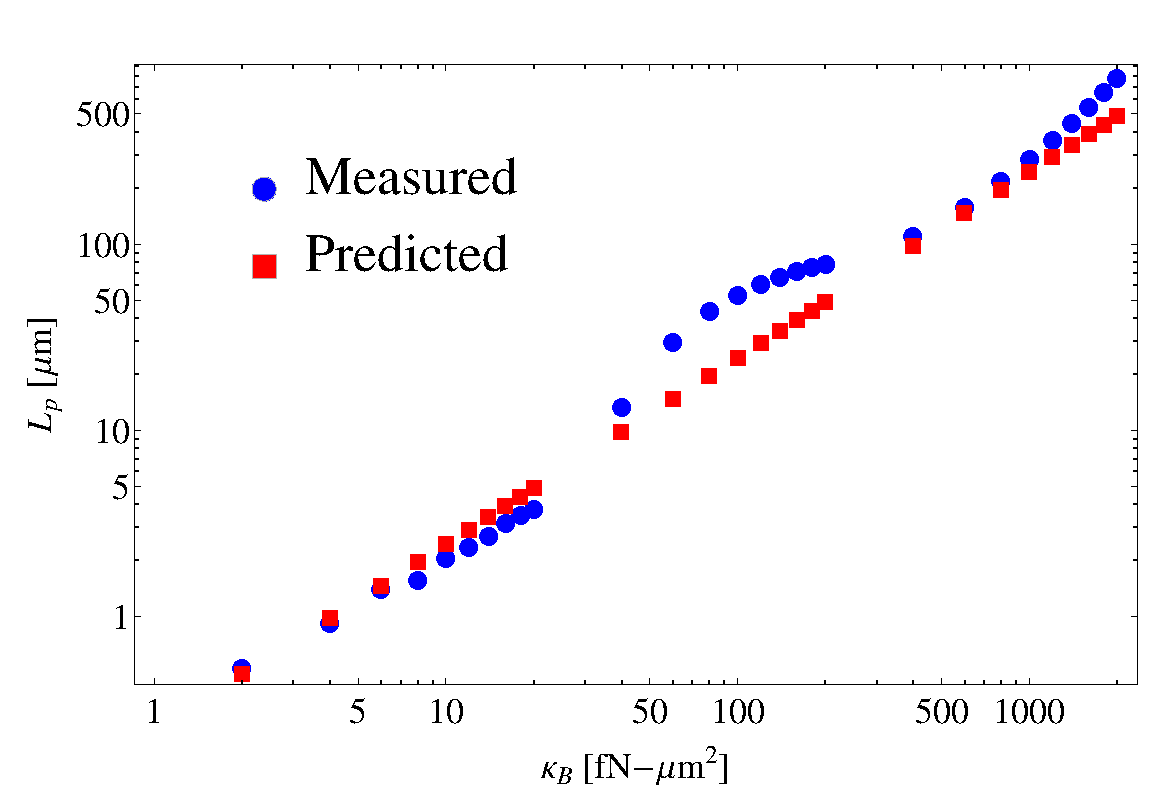
\includegraphics[width=\textwidth]{figs/filament/kb_vs_lp_fit_all.eps}
    \caption{\label{fig:kb}}
  \end{subfigure}
  ~
  \begin{subfigure}{0.4\textwidth}
    \centering
    \includegraphics[width=\textwidth]{figs/filament/kl_vs_lp_fit30.eps}
    \caption{\label{fig:kl}}
  \end{subfigure}%
  ~
  \begin{subfigure}{0.6\textwidth}
    \centering
    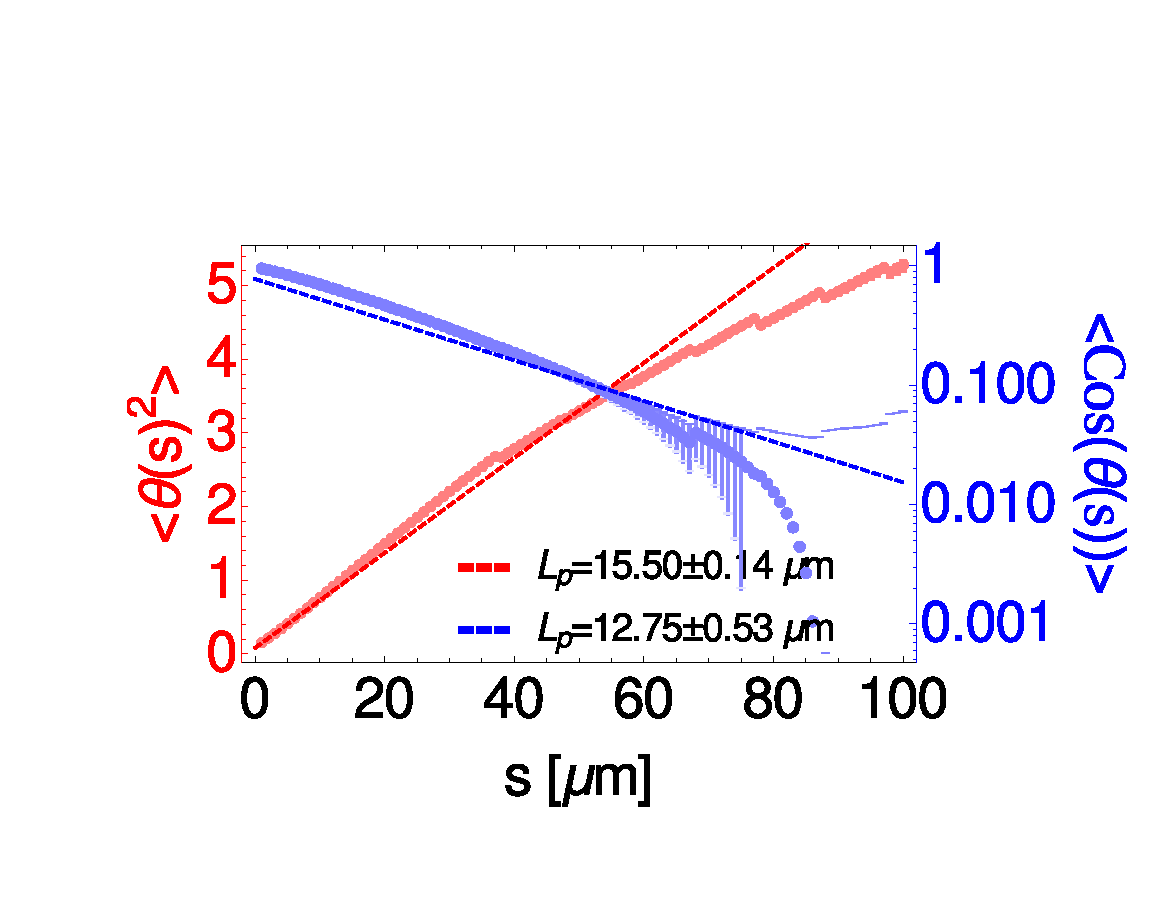
\includegraphics[width=\textwidth]{figs/filament/sAvgd_L1-100.eps}
    \caption{\label{fig:lp_vs_l}}
  \end{subfigure}
  ~
  \begin{subfigure}{0.4\textwidth}
    \centering
    \includegraphics[width=\textwidth]{figs/filament/R2vsL.eps}
    \caption{\label{fig:R2}}
  \end{subfigure}
  \label{fig:wlc_supp}
  \caption{
  \subref{fig:kb} Input bending modulus vs measured persistence length over three orders of magnitude. Persistence
  length was measured by fitting a line to $\ln{(\langle \cos{(\theta)}\rangle)}$ in each case.
    \subref{fig:kl}Persistence length as function of stretching stiffness approaches correct answer for high
  enough stiffness. 
  \subref{fig:lp_vs_l}Methods $1$ and $2$ of measuring persistence length, described in main text using different length
  filaments.
  \subref{fig:R2} A third method for measuring persistence length, as function of end to end distance, described above.
}
\end{figure}
\subsection{Strain Stiffening} \label{strain_supp} 
\begin{figure}[H] 
  \begin{subfigure}{0.35\textwidth}
    \centering
    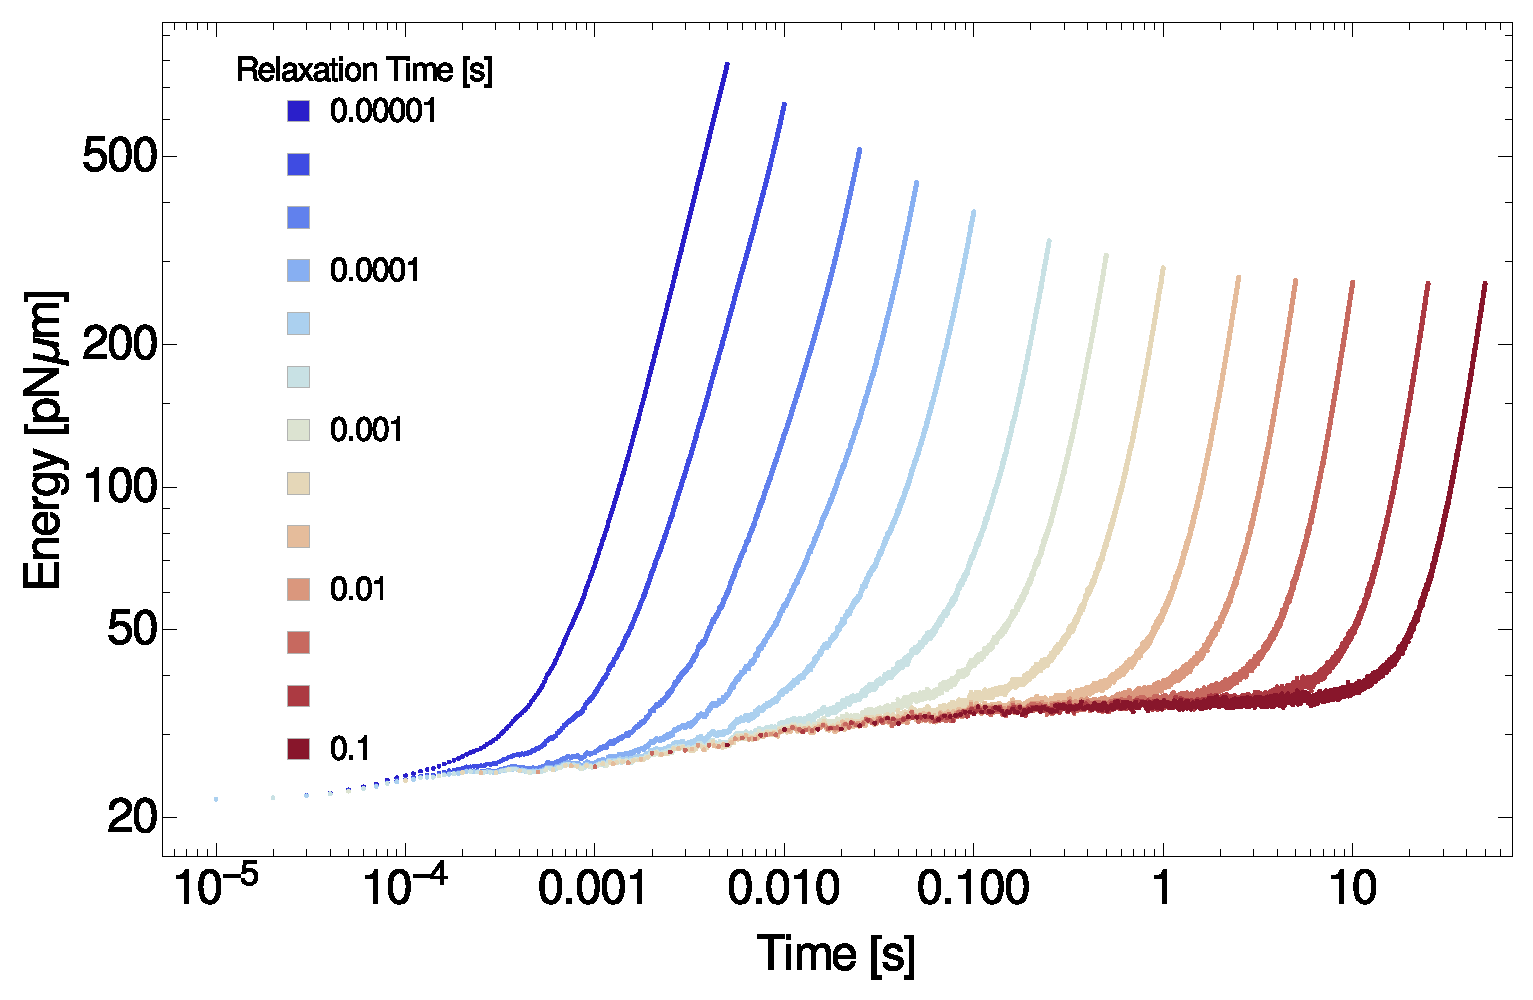
\includegraphics[width=\textwidth]{figs/elasticity/eng_vs_t_k10.eps}
    \caption{\label{fig:tRelax10}}
  \end{subfigure}
  \begin{subfigure}{0.35\textwidth}
    \centering
    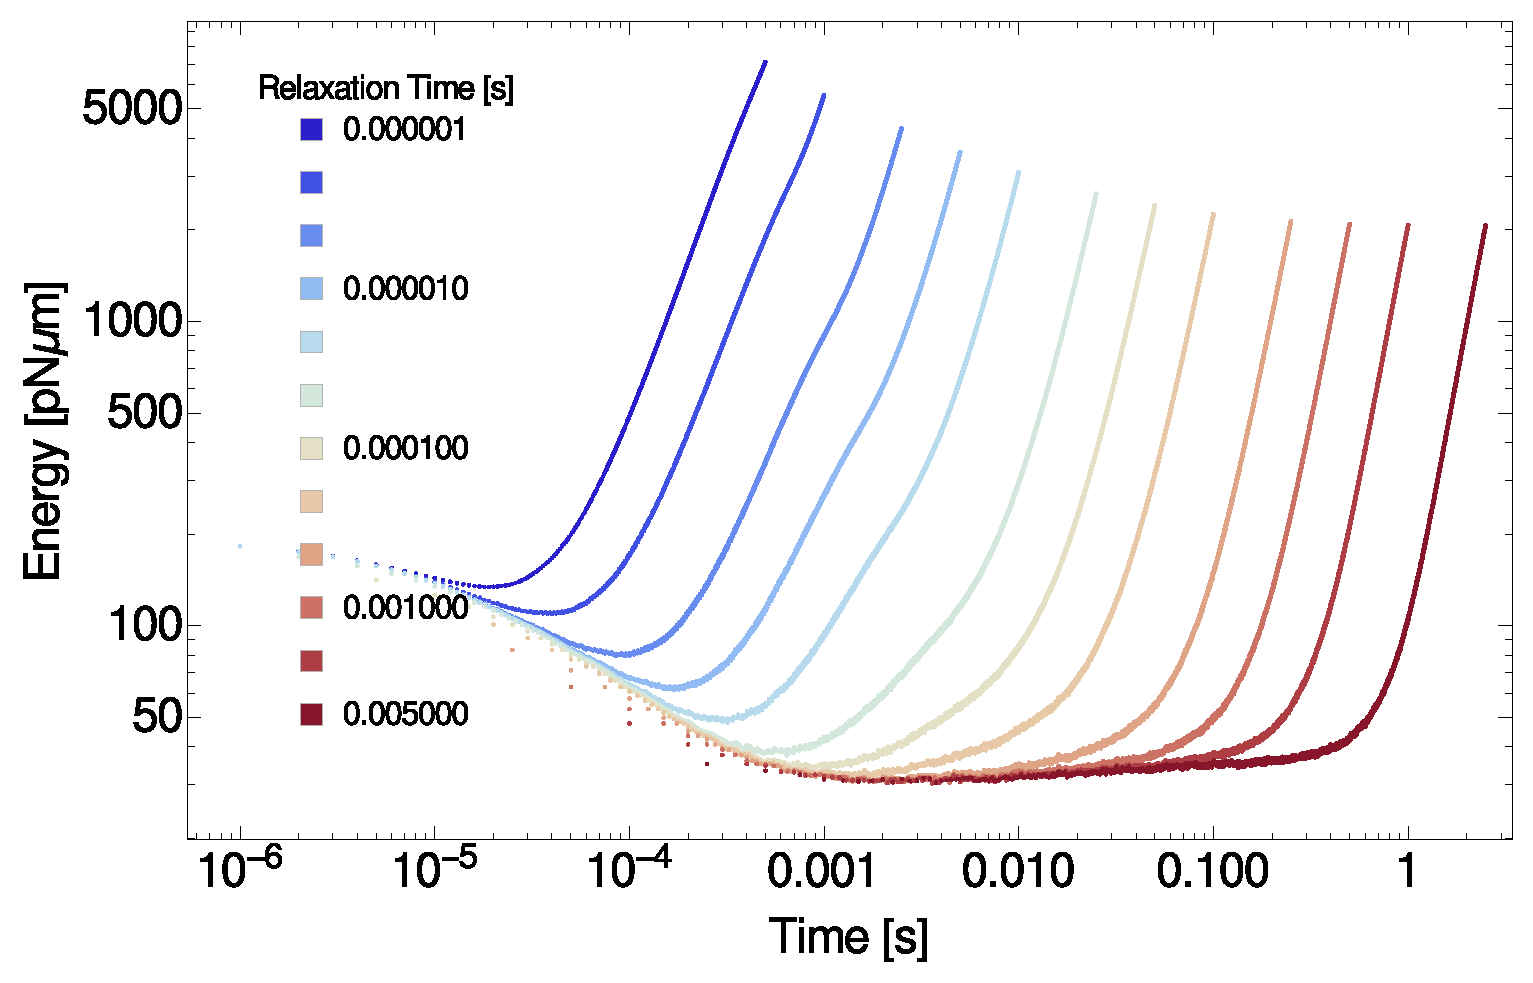
\includegraphics[width=\textwidth]{figs/elasticity/eng_vs_t_k100.eps}
    \caption{\label{fig:tRelax100}}
  \end{subfigure}
  \label{fig:tRelax}
  \caption{Strain energy as function of time for various relax times $t_\text{relax}$ for networks with 
  \subref{fig:tRelax10} $k_\text{cl}=10pN/\mu m$ and\subref{fig:tRelax100} $k_\text{cl}=100pN/\mu m$  
crosslinked networks}.
\end{figure}
\subsection{Bundling}
To contrast between bundling, contractility, and polarity sorting
we computed the divergence of bundled networks, as well as the
radial distribution function of the filament barbed ends in bundled
networks. The results are shown in figure \Cref{fig:bundling_supp}. 
\begin{figure}[H] 
  \centering
  \includegraphics[width=\textwidth]{figs/bundling/bundling_supplement.pdf}
  \caption{\label{fig:bundling_supp}
  (A) Assemblies without motors that bundle do not show an average negative divergence, unlike assemblies with motors (\Cref{fig:contract}).
  (B) The radial distribution function for bundled networks for the barbed end of filaments is significantly less peaked than for all points on the filaments (\Cref{fig:bundle}). Thus, the network is not polarity sorted. 
  }
\end{figure}
\end{document}
